\documentclass{article}
\usepackage[utf8]{inputenc}
\usepackage[spanish]{babel}
\usepackage{pdfpages}
\usepackage{listings}
\usepackage{graphicx}
\usepackage{float}
\usepackage{mips}


\setlength{\parskip}{1ex plus 0.5ex minus 0.2ex}
\title{Trabajo Práctico 1} 
\author{
  Agustin Alejandro Linari, \textit{Padrón Nro. 81.783}\\
  \textit{agustinlinari@gmail.com}\\
  \and
  Juan Ignacio López Pecora, \textit{Padrón Nro. 84.700}\\
  \textit{jlopezpecora@gmail.com}\\
  \and
  Pablo Daniel Sívori, \textit{Padrón: 84.026}\\  
  \textit{sivoridaniel@gmail.com}\\
  \\
  \normalsize{2$^{\circ}$ Cuatrimestre de 2016}                           \\
  \normalsize{66.20 Organizacion de Computadoras}                  \\
  \normalsize{Facultad de Ingenieria, Universidad de Buenos Aires} \\
}

%\newcommand{\ip}[2]{(#1, #2)}
                             % Defines \ip{arg1}{arg2} to mean
                             % (arg1, arg2).

%\newcommand{\ip}[2]{\langle #1 | #2\rangle}
                             % This is an alternative definition of
                             % \ip that is commented out.

\begin{document}             % End of preamble and beginning of text.

%\maketitle                   % Produces the title.
\maketitle


\begin{abstract}
En el presente trabajo utilizamos el conjunto de instrucciones MIPS y el concepto de ABI para resolver parte de la lógica del programa realizado en el trabajo práctico 0. 
\end{abstract}

\clearpage

\tableofcontents
\clearpage

\part{Desarrollo}

\section{Introduccion}

El objetivo del presente trabajo práctico es familiarizarse con el código de instrucciones MIPS 32. Para ello implementaremos la lógica de cómputo del fractal con dicho código de instrucciones. También durante el desarrollo del mismo haremos uso de la convención de llamada de funciones definida en la ABI de MIPS 32. Se hará uso de la syscall SYSwrite para realizar la impresión de los caracteres ascii sobre el archivo pgm. Para utilizar la syscall de manera eficiente se utilizará un buffer de tamaño parametrizable con el fin de reducir la cantidad de llamdas a la misma. Finalmente compilaremos el programa en el emulador GXemul para poder ejectuar el mismo en un sistema operativo NetBSD.

\section{Build}
El correspondiente informe se puede construir utilizando el make con la etiqueta doc la cual borra y genera el informe en formato pdf.

Para la compilación del trabajo práctico, copiar el directorio tp1 al emulador y luego ejecutar dentro del directorio tp1/src los siguientes comandos.

\begin{lstlisting}[language=bash]
 $ make clean
 $ make makefiles
 $ make
\end{lstlisting}

Para ejecutar las pruebas, en primer lugar realizar el build y luego desde el directorio tp1/test correr el script run-tests.sh.

\section{Diseño e Implementación del Programa}

El código fuente del programa se puede encontrar en el anexo \ref{sec:source}.

Para la implementación de la solución se codificaron cuatro funciones.


\subsection{Funciones de escritura}

Las funciones buff\_write y buff\_flush son las encargadas de administrar la impresión de los caracteres sobre el buffer y por lo tanto se encargan también de efectuar la syscall SYS\_write. Más precisamente, buff\_write utiliza un buffer de chars definido en una región .data de memoria y accedido mediante un indice también estático. Recibe como parámetros el file descriptor que indica a que archivo hay que imprimir, un char* con la secuencia de caracteres a escribir en el buffer y otro int para indicar el tamaño en bytes de esta secuencia.
La función buff\_flush es la encargada de efectuar la llamada a la syscall, mandando todo el buffer a imprimir y luego reiniciar su índice para poder seguir imprimiendo sobre el mismo. Recibe como parámetro el file descriptor.

A continuación mostramos el diagrama de stack frame de las mismas.

\begin{figure}[H]
	\centering
		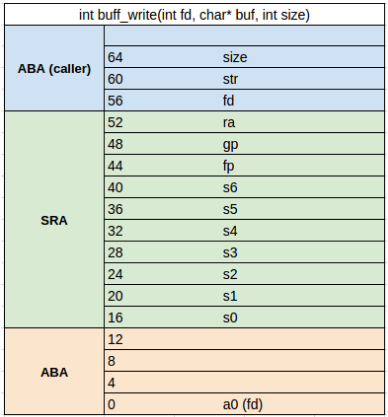
\includegraphics[scale=0.4]{stack1.png}
	\caption{Stack1}
	\label{fig:stack1}
\end{figure}

\begin{figure}[H]
	\centering
		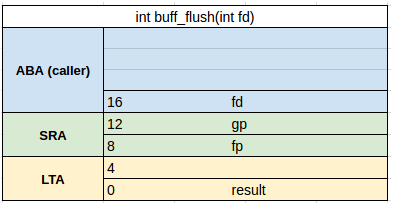
\includegraphics[scale=0.4]{stack2.png}
	\caption{Stack2}
	\label{fig:stack2}
\end{figure}

Como se puede observar en este caso optamos por hacer uso de los registros S, sin embargo, también podriamos haber utilizado variables locales y alojarlas en la LTA. Los registros S son almacenados en el SRA al iniciar la función y luego son restaurados a su valor original, de esta forma respetamos la ABI.

\subsection{Función para conversión de enteros a caracteres ascii}

Se necesito crear una función que realice la conversión de enteros a caracteres ascii y los imprima. En este caso, aprovechamos uno de los ejemplos brindados por el curso: la función print\_dnames.S. Tomamos como base la misma y la adaptamos para imprimir cada dígito como un caracter ascii.
La función la renombramos como:

int print\_int(unsigned int n, unsigned int fd)

Recibe como primer argumento el número a convertir y como segundo el file descriptor. La misma, a diferencia de la original, hace uso de las funciones buff\_write y buff\_flush para imprimir el número entero en el buffer.

A continuación mostramos el diagrama de stack frame de la misma.

\begin{figure}[H]
	\centering
		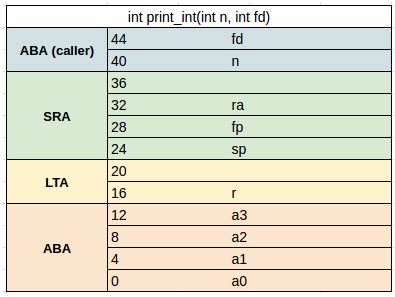
\includegraphics[scale=0.4]{stack3.png}
	\caption{Stack3}
	\label{fig:stack3}
\end{figure}

\subsection{Función generadora de fractal}

Por último, mostramos la función que contiene la lógica para generar el fractal e imprimirlo en un archivo con formato pgm:

int mips32\_plot(param\_t* params)

Esta función contiene la lógica principal para generar el fractal de Julia y hace uso de todas las funciones presentadas previamente. 

A continuación mostramos el diagrama de stack frame de la misma.


\begin{figure}[H]
	\centering
		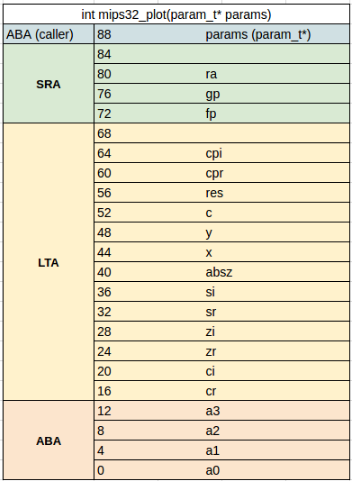
\includegraphics[scale=0.4]{stack4.png}
	\caption{Stack4}
	\label{fig:stack4}
\end{figure}

\clearpage

\subsection{Pruebas}

Se creó un script para la ejecución de diversos tests. El mismo se puede ubicar dentro de la carpeta test con el nombre run.test.sh. Junto a él, se pueden encontrar archivos pgm que fueron generados a partir de la ejecución de la versión C de mips32\_plot. Para poder correr el script es necesario que se haya realizado el build previamente.
El mismo correrá un set de pruebas, comparando las salidas para los siguientes casos:

Caso default

\begin{lstlisting}[language=bash]
 $ ./tp1 -o out.pgm;
\end{lstlisting}

Caso punto perteneciente a conjunto de Julia

\begin{lstlisting}[language=bash]
 $ ./tp1 -c 0.01+0i -r 1x1 -o out.pgm;
\end{lstlisting}

Caso punto no perteneciente a conjunto de Julia

\begin{lstlisting}[language=bash]
 $ ./tp1 -c 10+0i -r 1x1 -o out.pgm;
\end{lstlisting}

Caso de prueba 1 variando constante C

\begin{lstlisting}[language=bash]
 $ ./tp1 -C 0.285+0i -o out.pgm;
\end{lstlisting}

Caso de prueba 2 variando constante C

\begin{lstlisting}[language=bash]
 $ ./tp1 -C -0.8+0.156i -o out.pgm;
\end{lstlisting}

Caso de prueba 3 variando constance C

\begin{lstlisting}[language=bash]
 $ ./tp1 -C 0+0.8i -o out.pgm;
\end{lstlisting}

Caso de prueba idem 2 pero con zoom sobre una región

\begin{lstlisting}[language=bash]
 $ ./tp1 -C -0.8+0.156i -w 0.5 -H 0.5 -o out.pgm;
\end{lstlisting}

\clearpage


\section{Corridas de Programa}

Se corre el programa obteniendose los siguientes tiempos de ejecución que se detallan en los siguientes cuadros.

\begin{table}[htbp]
\begin{center}
\begin{tabular}{|l|l|l|l|}
\hline
Código C & real & usr & sys \\
\hline \hline
1 & 1m19.363s & 1m19.143s & 0m0.141s \\ \hline
2 & 1m23.195s & 1m23.014s & 0m0.129s \\ \hline
3 & 1m21.480s & 1m19.335s & 0m0.133s \\ \hline
promedio & 1m 21.346s & 1m 20.497s & 0.134s
\end{tabular}
\caption{Tiempos promedios de ejecución en código C.}
\end{center}
\end{table}

\begin{table}[htbp]
\begin{center}
\begin{tabular}{|l|l|l|l|}
\hline
Código C & real & usr & sys \\
\hline \hline
1 & 1m0.449s & 0m52.722s & 0m7.680s \\ \hline
2 & 1m0.879s & 0m53.042s & 0m7.808s \\ \hline
3 & 1m1.246s & 0m53.261s & 0m7.937s \\ \hline
promedio & 1m0.858s & 53.008s & 7.808s
\end{tabular}
\caption{Tiempos promedios de ejecución en código Mips buffer size 64 bytes.}
\end{center}
\end{table}

\begin{table}[htbp]
\begin{center}
\begin{tabular}{|l|l|l|l|}
\hline
Código C & real & usr & sys \\
\hline \hline
1 & 1m4.262s & 1m3.237s & 0m0.984s \\ \hline
2 & 1m1.246s & 1m0.319s & 0m0.883s \\ \hline
3 & 0m58.547s & 0m57.573s & 0m0.937s \\ \hline
promedio & 1m1.352s & 1m0.376s & 0.935s
\end{tabular}
\caption{Tiempos promedios de ejecución en código Mips buffer size 1 KB.}
\end{center}
\end{table}

\begin{table}[htbp]
\begin{center}
\begin{tabular}{|l|l|l|l|}
\hline
Código C & real & usr & sys \\
\hline \hline
1 & 1m3.797s & 1m3.589s & 0m0.156s \\ \hline
2 & 1m0.617s & 1m0.480s & 0m0.133s \\ \hline
3 & 1m4.500s & 1m4.249s & 0m0.215s \\ \hline
promedio & 1m2.971s & 1m2.772s & 0.168s
\end{tabular}
\caption{Tiempos promedios de ejecución en código Mips buffer size 16 KB.}
\end{center}
\end{table}

\begin{figure}
\begin{itemize}
\item Todos los programas fueron compilados con el parámetro -O0 (sin optimizaciones).
\item Todas las mediciones corresponden a la ejecución de los programas utilizando el comando time.
\end{itemize}
\end{figure}



\begin{figure}[H]
\textit{\textbf{Representamos gráficamente los valores obtenidos en los cuadros anteriores, y hacemos una comparación entre los tiempos promedios de ejecución obtenidos en cada código}}\\
	\centering
		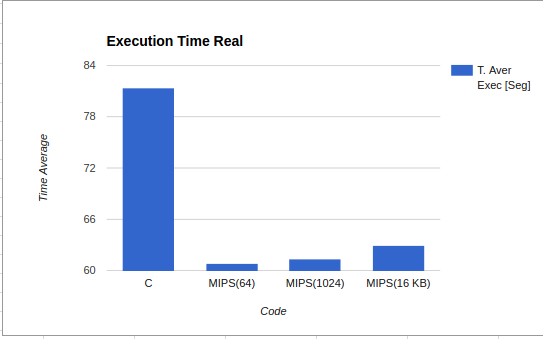
\includegraphics[scale=0.6]{TPromExecReal.png}
\end{figure}
\begin{figure}[H]
	\centering
	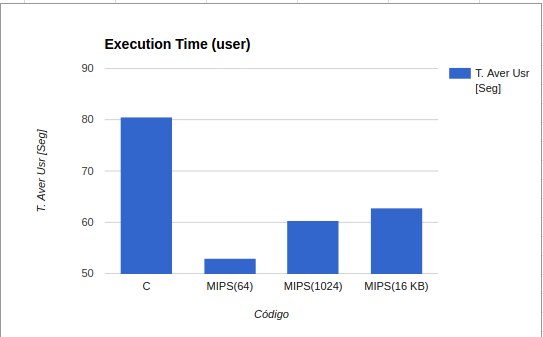
\includegraphics[scale=0.6]{TPromExecUsr.png}
\end{figure}
\begin{figure}[H]
	\centering
		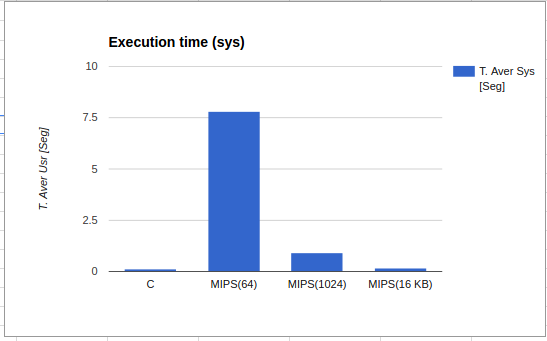
\includegraphics[scale=0.6]{TPromExecSys.png}
\end{figure}




\clearpage


\begin{table}[htbp]
\begin{center}
\begin{tabular}{|l|l|}
\hline
Speed Up & Value \\
\hline \hline
tc / tmips 64B & 1.34 \\ \hline
tc / tmips 1KB & 1.33 \\ \hline
tc / tmips 16KB & 1.29 \\ \hline

\end{tabular}
\caption{Speed UP}
\end{center}
\end{table}

\subsection{Observaciones}
\begin{itemize}
\item La implementación de mips en cualquiera de sus variantes se ejecuta en menos tiempo que la implementación C pura, con un speed up aproximado de 1/3
\item A medida que el buffer se agranda, el tiempo de sistema se reduce. Esto se debe a que se producen menos syscalls a write.
\item Podemos plantear la hipótesis razonable de que printf está implementada con un buffer (debido al bajo sys time). Para nuestra implementación MIPS, el tamaño del buffer que obtuvo un tiempo sys del mismo orden que la implementación C fue de 16 KB.
\item Contrario a lo que nuestra intuición indicaba, aumentar el buffer para valores mayores a 64 bytes no necesariamente significó (en promedio) en un aumento de performance. Esto puede estar relacionado con la arquitectura del cache emulado, el tamaño de bloque  y su política de reemplazo.
\end{itemize}

\clearpage
\subsection{Conclusión}


Con la realización de este trabajo hemos podido apreciar la diferencia de performance entre dos implementaciones de distinta naturaleza de un mismo algoritmo, implementado en C y en assembly MIPS32.


A la hora de programar, es común que se codifique utilizando lenguajes de alto nivel. El lenguaje de programación C es un lenguaje de propósito general clásico cuyo diseño provee construcciones que mapean de manera eficiente instrucciones de máquina típicas. Las ventajas de utilizar un lenguaje de alto nivel como C son portabilidad (a nivel código fuente) entre diferentes arquitecturas donde se haya implementado el compilador, aumento de productividad - dado que se abstrae de cuestiones de bajo nivel íntimamente ligadas con la arquitectura de la máquina - y reducción en el costo de mantenimiento. Sin embargo, estas ventajas traen aparejado un costo en la performance del programa.


En algunos casos, los requerimientos funcionales de un programa requieren de una performance que puede ser difícil de alcanzar para una implementación en un lenguaje de alto nivel. Mediante un análisis cuantitativo, se determina qué segmentos de código consumen la mayor cantidad de recursos de una computadora -ciclos de CPU, memoria, etc-. Para el caso particular de este trabajo, la función de cómputo del fractal es central en el desempeño de la aplicación.


\clearpage

\part{Apendice}
\appendix


\section{Codigo fuente}\label{sec:source}
\definecolor{gray}{rgb}{0.5,0.5,0.5}
\lstset{%
  language=[mips]Assembler,       % the language of the code
  basicstyle=\footnotesize,       % the size of the fonts that are used for the code
  numbers=left,                   % where to put the line-numbers
  numberstyle=\tiny\color{gray},  % the style that is used for the line-numbers
  stepnumber=1,                   % the step between two line-numbers. If it's 1, each line 
                                  % will be numbered
  numbersep=5pt,                  % how far the line-numbers are from the code
  backgroundcolor=\color{white},  % choose the background color. You must add \usepackage{color}
  showspaces=false,               % show spaces adding particular underscores
  showstringspaces=false,         % underline spaces within strings
  showtabs=false,                 % show tabs within strings adding particular underscores
  frame=single,                   % adds a frame around the code
  rulecolor=\color{black},        % if not set, the frame-color may be changed on line-breaks within not-black text (e.g. commens (green here))
  tabsize=4,                      % sets default tabsize to 2 spaces
  captionpos=b,                   % sets the caption-position to bottom
  breaklines=true,                % sets automatic line breaking
  breakatwhitespace=false,        % sets if automatic breaks should only happen at whitespace
  title=\lstname,                 % show the filename of files included with \lstinputlisting;
                                  % also try caption instead of title
  keywordstyle=\color{blue},      % keyword style
  commentstyle=\color{green},     % comment style
  stringstyle=\color{red},      % string literal style
  escapeinside={\%*}{*)},         % if you want to add a comment within your code
  morekeywords={*}                % if you want to add more keywords to the set
}


\lstinputlisting{../src/mips32_plot.S}
\lstinputlisting{../src/print_int.S}
\lstinputlisting{../src/buff_write.S}

\clearpage

\section{Enunciado original}\label{sec:enunciado}
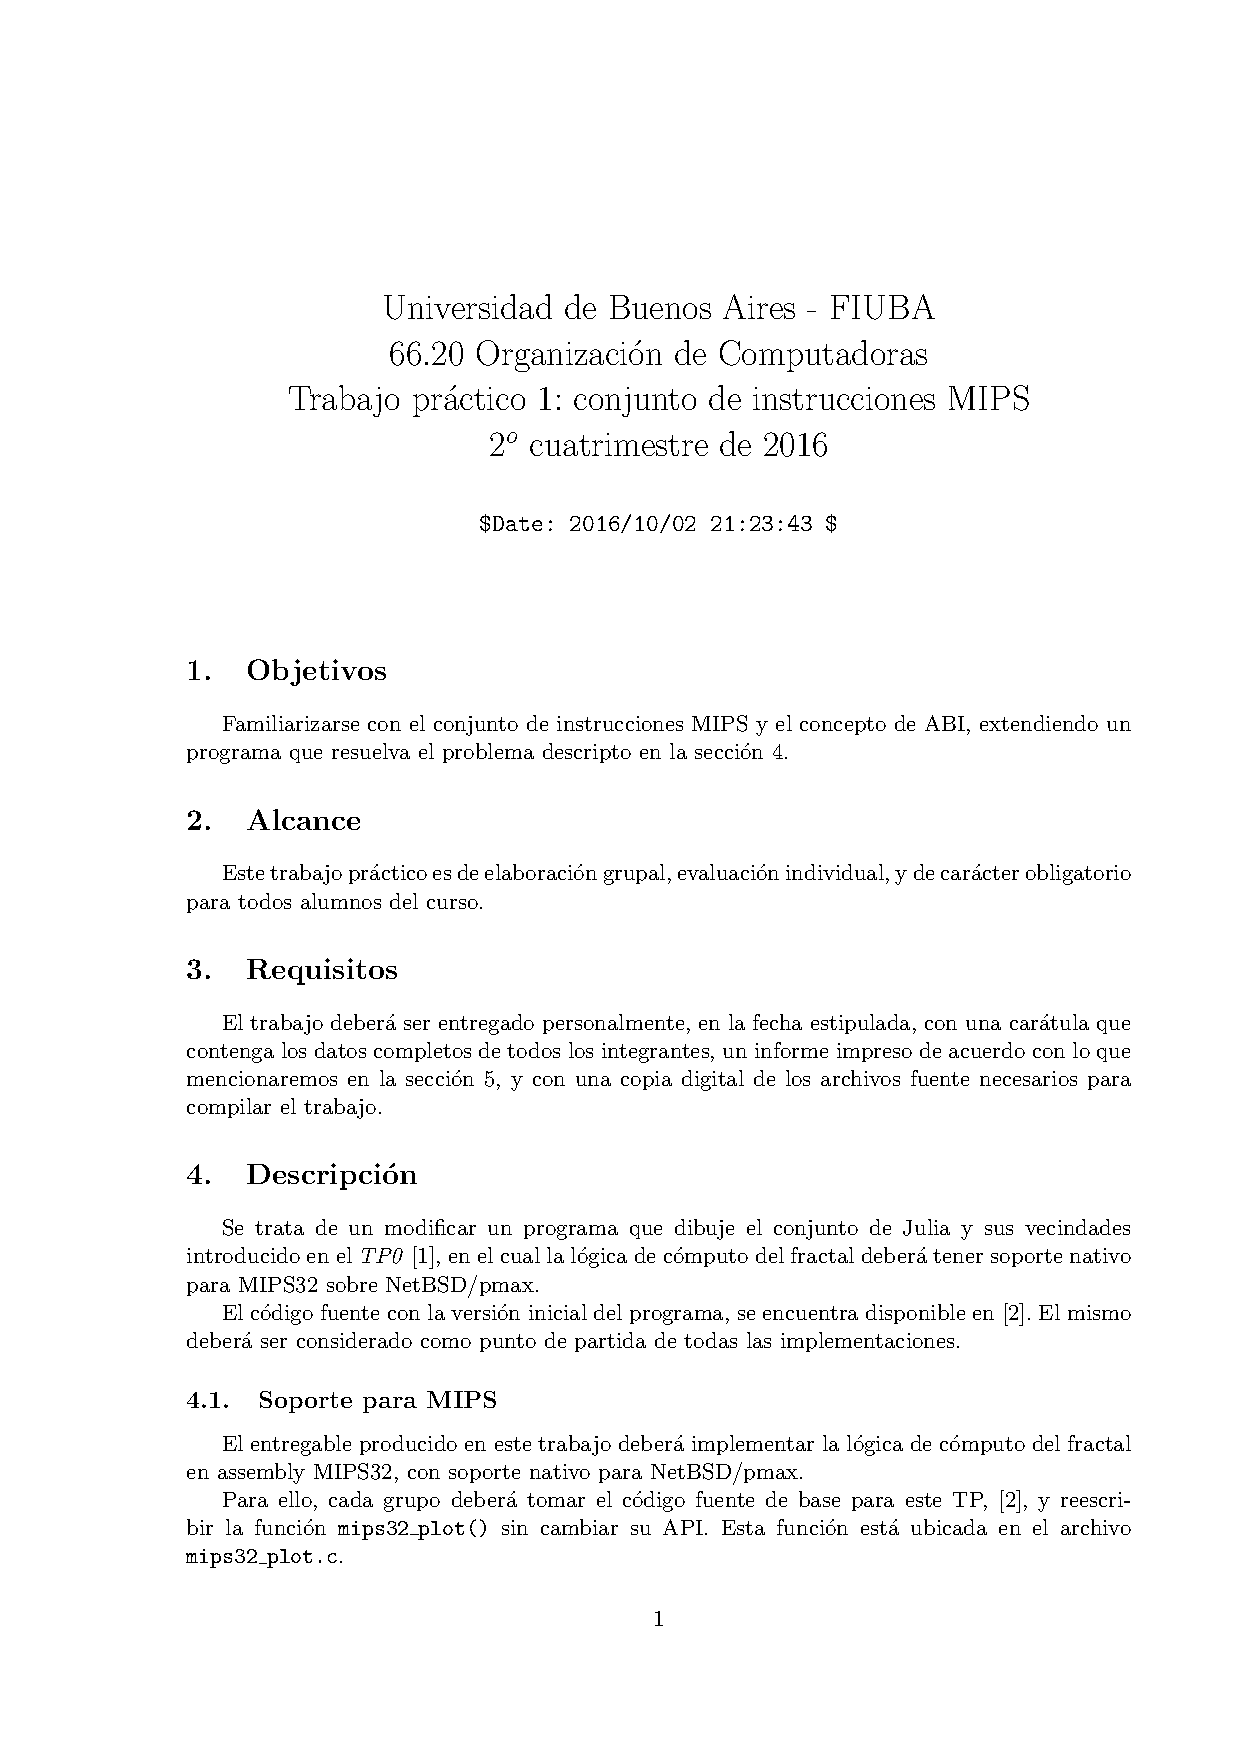
\includepdf[pages={-}]{tp1-2016-2q.pdf}

\end{document}               % End of document.
